%\vspace{-20pt}
\section*{Abstract}
The growth in SSD capacity is reaching its limit 
due to the stunted growth of capacitors---electrical components that store charge 
to protect data for the volatile memory in case of power loss. 
While the SSD's capacity scaled from 256GB in 2011~\cite{samsung2011} to 30TB in 2018~\cite{anandtech18samsung} (100$\times$), 
the density of Aluminum and Tantalum electrolytic capacitors only by tenfold from 1960 to 2005~\cite{both2015modern}.
This slow scaling will eventually limit the amount of DRAM that can be used in an SSD,
and this, in turn, will also limit the storage capacity as the size of DRAM and aggregate flash capacity proportionally scale~\cite{samsung_ratio, ni2017hash}. 

\iffalse
Enterprise-class SSDs provide a persistent internal buffer using the capacitors. 
This PLP(Power-Loss Protection) mechanism reached a limit as the SSD density outpaces the scaling capability of the capacitors. 
% The SSD has increased significantly in density for the past decade. 
% With the growing popularity of data-intensive applications, the SSD density has increased rapidly in recent years.
%, expanding by 100× over the past ten years [1], [15].
% As an example, 
In 2011, a typical 2.5-inch SSD had 256GB capacity, but
%the world's first 2TB SSD was released in 2013~\cite{foremay2013}, but 
by 2018, a high-capacity SSD boasted a 30TB, expanding by 100× over the past ten years
~\cite{samsung2011, anandtech18samsung}. 
\begin{comment}
This remarkable growth of the device-capacity is thanks to the advanced scaling technologies 
such as nanoscale fabrication~\cite{busche2014design} and multi-layer stacking~\cite{9365809}. 
\end{comment}
% As an example, in 2011, a typical 2.5-inch SSD had 256GB capacity with 256MB of DRAM; by 2018, a high-capacity 2.5- inch SSD boasted a 30TB with 40GB of
% Unfortunately, not all components of the SSDs have kept up with the scaling rate.
However, the capacitor fails to proceed at the pace. 
\begin{comment}
Historically, storage devices 
have been equipped with a small size of volatile buffer in front of the persistent disk. 
By using them as a write buffer, they hide a long latency of the physical storage medium 
as well as mitigating an endurance limitation of the worn-out devices. 
However, the volatile buffer loses all data in the event of power crash. 
To prevent a data loss or corruption by this, enterprise-class SSDs
rely on the capacitors; it reserves energy to persist data in volatile buffer 
in the unforeseen event of a power crash. 
In addition, the adoption of capacitors enables an SSD to ignore the \texttt{FLUSH} command that explicitly requests all data in the volatile buffer to be made durable.
This property increases the buffering effect in SSD significantly, leading to both less write traffic and a shorter operation latency.
% To overcome this limitation without sacrificing performance, 
The reliance on capacitors, however, has reached its limit. 
\end{comment}
% the improvement in capacitance fails to keep up with the rapid growth of SSDs. 
%Al(aluminum) and Ta(tantalum)-electrolytic capacitors used in SSDs have increased in density through miniaturization by tenfold from 1960 to 2005 [4]. 
The capacitance density has also steadily improved, but
it is not as rapid as the SSD scaling speed. 
Al(aluminum) and Ta(tantalum)-electrolytic capacitors used in SSDs 
have increased in density by tenfold from 1960 to 2005~\cite{both2015modern}. 
This is approximately 50x slower than the SSD density increase rate.
Given that the internal buffer size increases in proportion to the storage capacity (typically 0.1\% of storage capacity~\cite{samsung_ratio, ni2017hash}),
the density gap between capacitance and memory technologies 
imposes an intrinsic limitation on the current architecture wherein 
the entire buffer is protected by capacitors. 
\fi

This paper presents a device-internal buffer architecture called \ours{} 
for the SSDs under capacitance constraints. 
% which operates under capacitance constraints.
% Fig.~\ref{fig_dawid_archi} shows the SSD architecture targeted in our study. 
\iffalse
\textcolor{blue}{
Historically, storage devices have been equipped with a small size of volatile buffer in front of the persistent disk. By using them as a read cache and a write buffer, they hide a long latency of the physical storage medium as well as mitigating an endurance limitation of the worn-out devices.
However, the volatile buffer loses all data in the event of power crash. 
To prevent a data loss or corruption by this, enterprise-class SSDs
rely on the capacitors; it reserves energy to persist data in volatile buffer 
in the unforeseen event of a power crash. 
In addition, the adoption of capacitors enables an SSD to ignore the \texttt{FLUSH} command that explicitly requests all data in the volatile buffer to be made durable.
This property increases the buffering effect in SSD significantly, leading to both less write traffic and a shorter operation latency.
% \EUNJI{Need to make this part shorter}
}
\fi
% To overcome this limitation without sacrificing performance, 
% The reliance on capacitors, however, has reached its limit. 
\ours{} achieves a persistent buffer with small size of capacitance by answering the following two questions. 
%(1) what not to protect under capacitance limitation and (2) how to reduce the overhead of ensuring persistence for unprotected data.
First question is \textit{what not to protect under capacitance constraints}. The device-internal buffer is used for (1) caching translation information (i.e., mapping index) and (2) buffering user writes. 
% The data maintained in the buffer can be classified into two types: the actual user data and 
% the metadata for SSD management (i.e, mapping table). 
\ours{} applies the capacitance constraints only to translation information, while protecting the user data entirely. The user data write is synchronous with the user request and unrecoverable upon a power outage. It hampers user experiences seriously when unprotected. On contrary, 
translation information is entirely managed by the firmware and provides room for compromise when SSDs suffer from capacitance restriction. \EUNJI{Furthermore, the main culprit demanding buffer space is translation information because a flat structured table is widely used for its indexing and has a large memory footprint.} 
Second question is thus \textit{how to reduce the cost of ensuring persistence for the translation updates}. When the buffer is partially protected, the number of dirty pages is limited to the maximum amount of data that the on-board capacitance can protect. If it goes beyond the limit, changes should be immediately flushed to the flash memory. \ours{} mitigates the negative impact of this behavior with a capacitance-contraint aware I/O scheduling.
%to meet the durability constraint for SSDs. XX mapping table XX flush 줄여보자.

% otherwise durability violated. 
% \EUNJI{
% 보호되지 못하는 데이터가 있을 때 버퍼를 어떻게 관리하면, 보호되지 못하는 데이터의 persistence 를 유지하기 위해 발생하는 비용을 적게 발생시킬 것인가? 에 대한 질문. }
% \EUNJI{제안하는 기법: 부분적으로 보호되는 맵핑 테이블의 동기화 오버헤드를 줄이기 위해, 해당 비용을 최소로 증가시키도록 I/O 스케줄링을 하는 것임.}

%\section{Design of \ours{} Buffer}
% \section{Least Increase of Dirtiness Scheduling}
A primary way of  reducing the superfluous writes caused by a capacitance limitation is to maintain the dirty memory footprint below a protected threshold as long as possible. When a dirty page overflow occurs, flushing is forced and write amplification increases.
% The \ours{} buffer aims at minimizing the dirty memory footprint of the mapping table at any point in time.
To this end, \ours{} aggregates and batches the requests whose mapping entry resides in the same page. \EUNJI{This policy reduces the dirty memory footprint of the mapping table at any point in time, amortizing the synchronization overhead across more requests. As such, \ours{} delivers less write traffic and higher IOPS than existing scheduling (e.g., FIFO) under capacitance constraints. \ours{} maintains two data structures: \textit{a zero-cost list} that holds the write requests whose mapping table page is in dirty state, and \textit{a max binary heap} that maintains the mapping table page indexes sorted by the number of associated write requests. 
% We term this policy Least Increase of Dirtiness (LID) scheduling.
When NAND flash becomes idle, \ours{} sends a request from the (1) zero-cost list first and if it is empty, (2) from the max binary heap. 
}  
\iffalse
In this regard, the \ours{} buffer aims at minimizing the \textit{dirty memory footprint} of the mapping table at any point in time. To this end, \ours{} processes outstanding requests in the order that least increases the number of dirty pages in the mapping table. 
This scheme not only reduces the number of flushes for the mapping table partially protected but also increases the efficiency of flush operation by aggregating more translation updates into the smaller translation pages.
\fi

\iffalse
because (1) the data write is synchronous with the user request and (2) the user data takes up a relatively 
small footprint in the buffer. 
\fi
% This is because the storage suffers from serious performance degradation when the user data 
% is not fully protected and should be entirely flushed upon a \texttt{FLUSH} command.
% }
% \textcolor{brown}{
% \ours{} essentially limits the number of dirty pages within buffer
% to the level the maximum capacitance can protect.
% If the number of dirty pages goes beyond the limit, changes are flushed to the flash memory. 
% }
% \EUNJI{For this architecture, the problem boils down to how to reduce the write traffic to persist the mapping table to flash memory under capacitance constraints.
% \iffalse
Reducing the synchronization overhead of the mapping table is a well-known problem and has been extensively studied for a past decade~\cite{jiang2011s, kim2017shrd}. 
However, they mostly focus on the SSDs without PLP, which have different properties to the PLP-SSDs with capacitance constraints. 

\EUNJI{\ours{} is built upon the current trend of increasing queue depth of the storage interfaces. SATA and SAS support a single queue with 32 and 245 commands, but NVMe has 
up to 65,535 queues with as many as 65,536 commands per queue. 
This extension allows SSDs to further optimize the internal activities by taking advantage of the outstanding request information.
}

We implement \ours{} in \texttt{FEMU}, an open-source SSD development framework~\cite{li2018case}. Fig. XX shows that \ours{} reduces the write traffic by up to 78\% and provides 25\% higher IOPS 
compared to the FIFO scheduling when only 10\% of the mapping table is protected. 
Compared to the full-protection architecture, \ours{} has has 20\% more writes and 
9\% of performance overhead, while reducing the required capacitance by 90\%. 
Fig.XX shows 
\iffalse
To evaluate the effectiveness of \ours, we implement the proposed buffer design
in \texttt{FEMU}, which is an open-source SSD development framework~\cite{li2018case}. The performance evaluation with various workloads 
shows that \ours{} reduces the write traffic by up to 78\% and provides 25\% higher IOPS 
compared to the FIFO scheduling scheme when only 10\% of the mapping table is protected. 
Compared to the full-protection architecture, \ours{} has has 20\% more writes and 
9\% of performance overhead, while reducing the required capacitance by 90\%. 
\fi

\begin{figure}[t]
    \centering{}
    \includegraphics[width=0.20\textwidth]{shn-graph/rand-wt.eps}
    \includegraphics[width=0.20\textwidth]{shn-graph/rand-iops.eps}
    %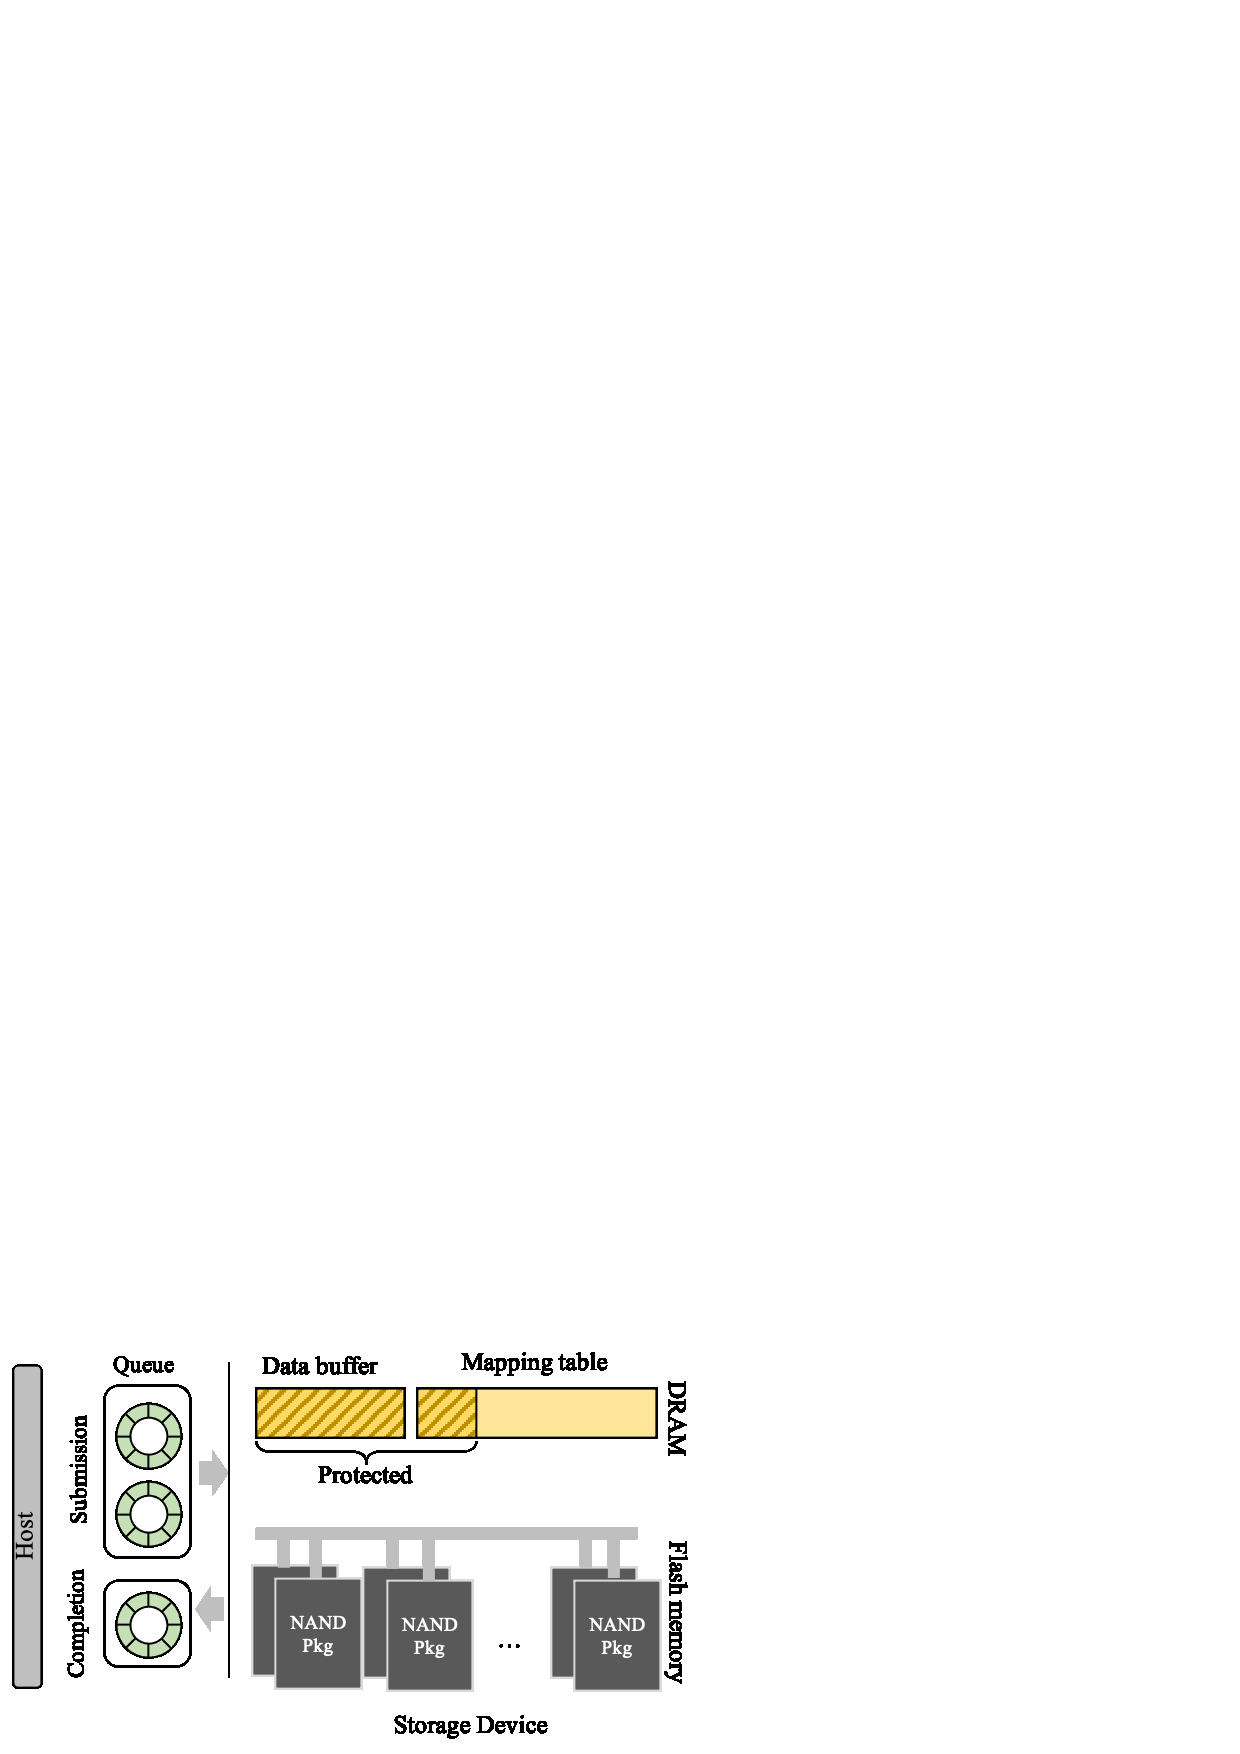
\includegraphics[width=0.4\textwidth]{figure/dawid_ssd_archi.png}
    \caption{\textbf{Write Traffic and IOPS (FIO-RAND).}}
    \label{fig_dawid_archi}
\end{figure}

\begin{figure}[t]
    \centering{}
    \includegraphics[width=0.20\textwidth]{shn-graph/jesd-wt.eps}
    \includegraphics[width=0.20\textwidth]{shn-graph/jesd-iops.eps}
    %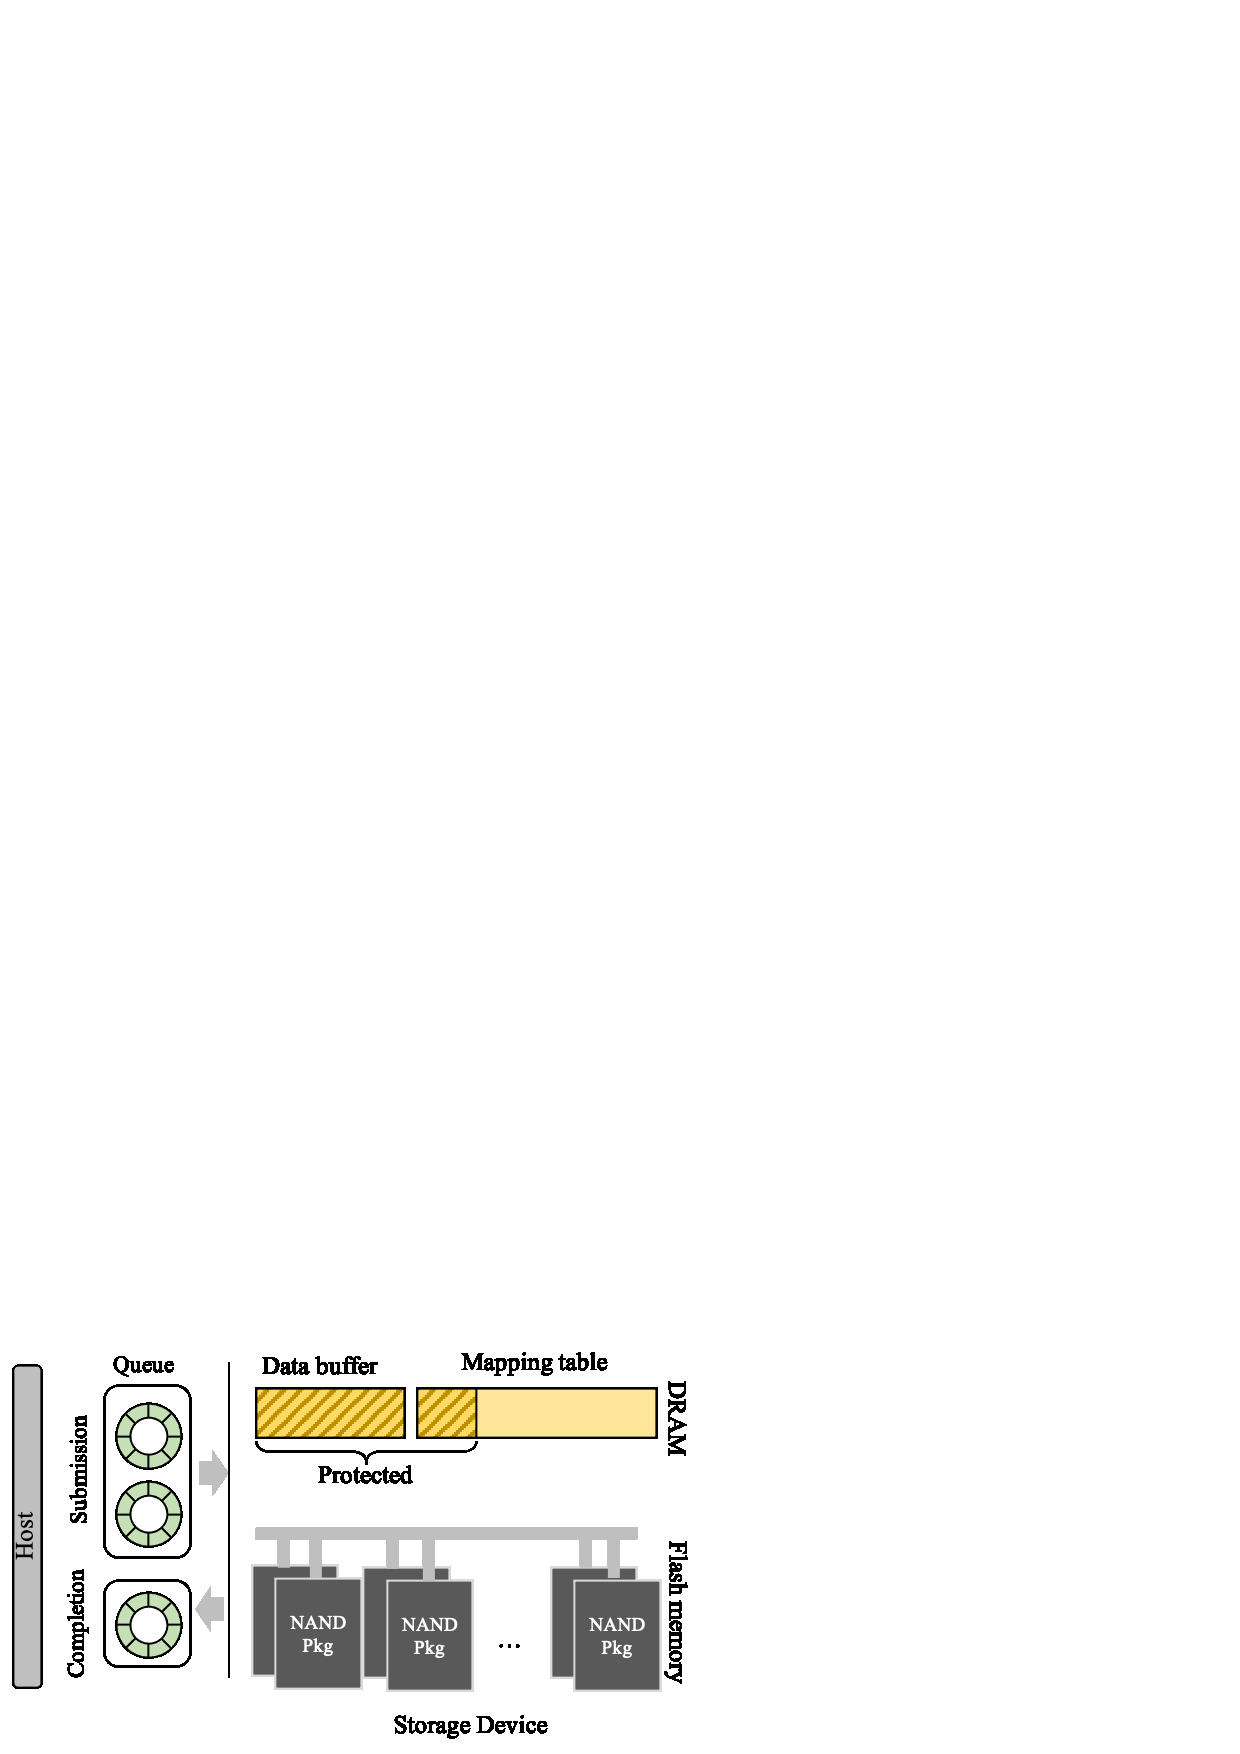
\includegraphics[width=0.4\textwidth]{figure/dawid_ssd_archi.png}
    \caption{\textbf{Write Traffic and IOPS (FIO-JESD) .}}
    \label{fig_dawid_archi}
\end{figure}

% \begin{figure}[t]
%     \centering{}
%     \includegraphics[width=0.5\textwidth]{figure/iops_write_traffic.png}
%     %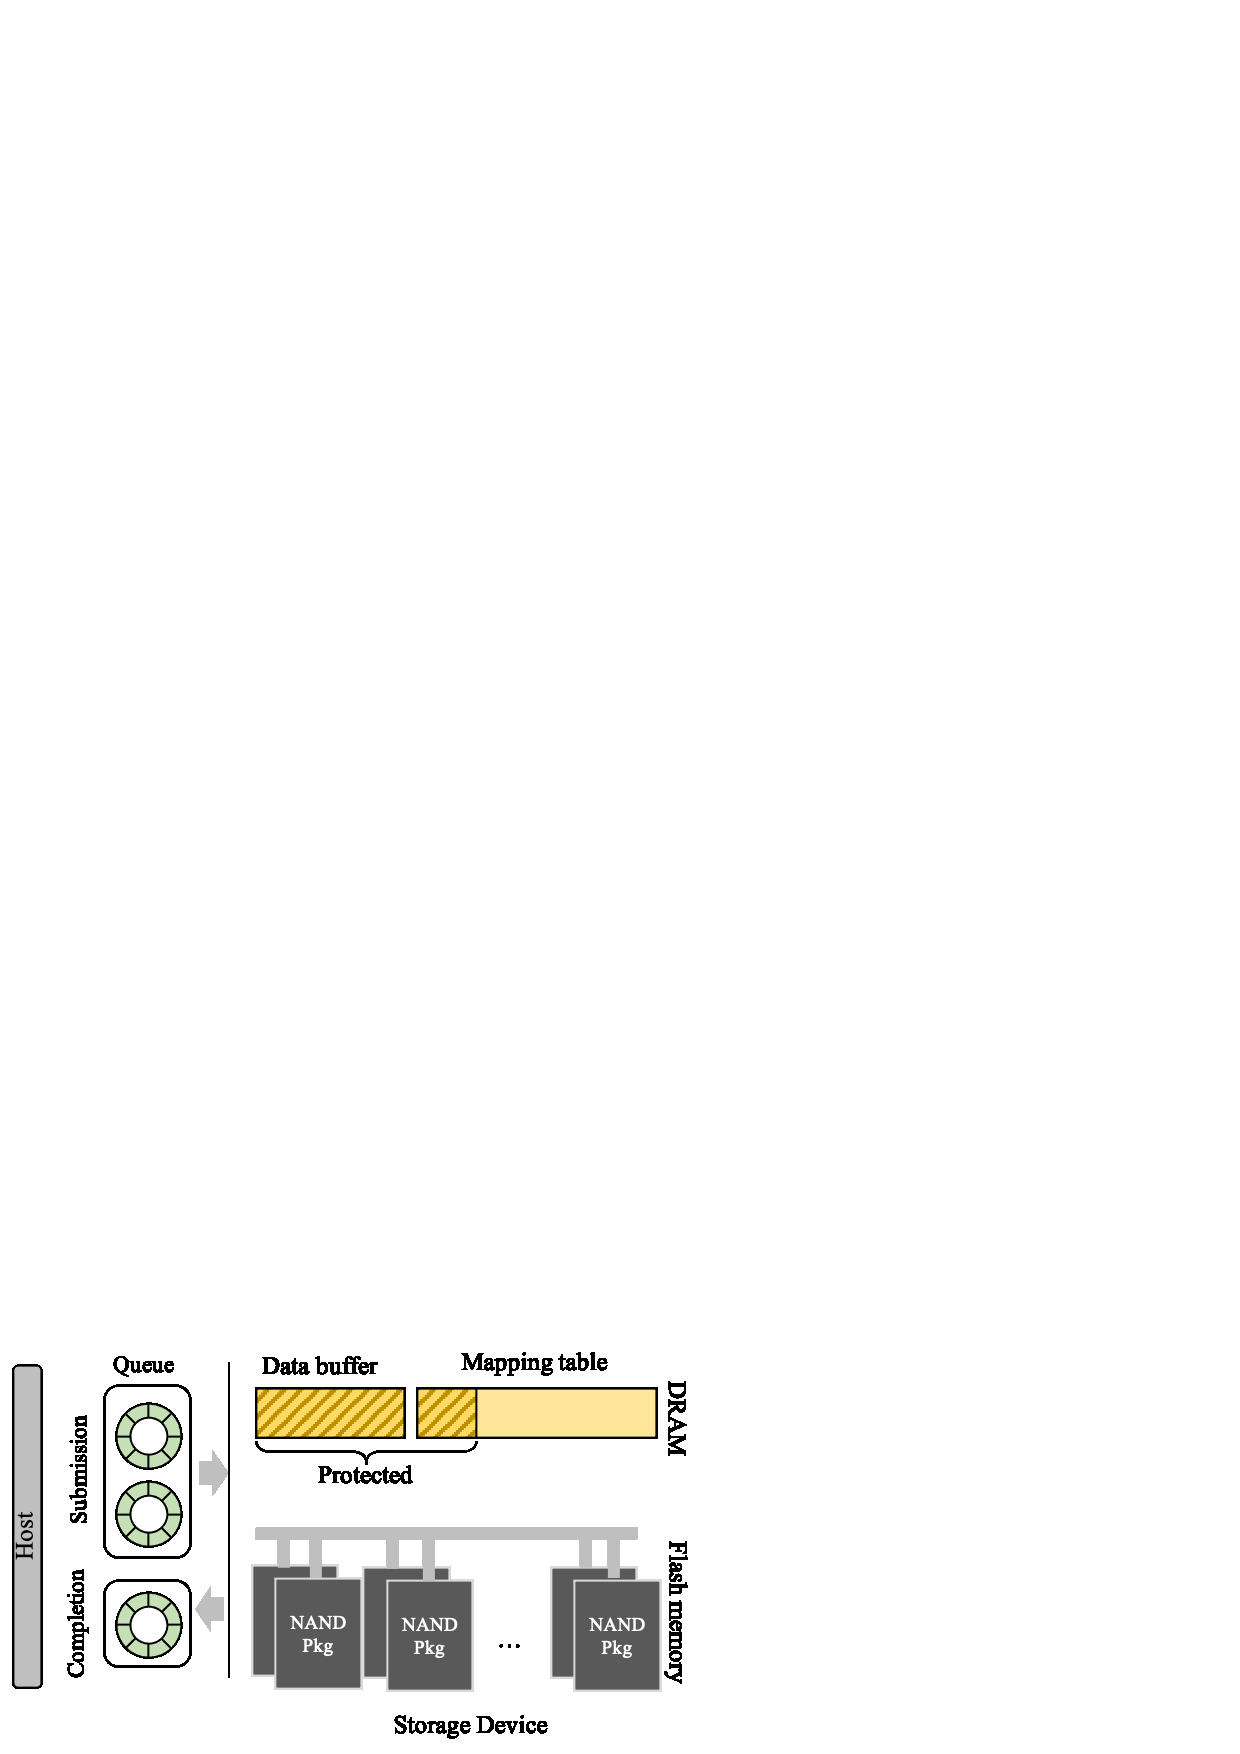
\includegraphics[width=0.4\textwidth]{figure/dawid_ssd_archi.png}
%     \caption{\textbf{IOPS and Write Traffic.}}
%     \label{fig_dawid_archi}
% \end{figure}
